\chapter{FEA data management}
\label{chapter:data-management}

Together with growing complexity of finite element calculations, the importance of management of data produced by the calculations is increasingly emphasized in both industrial and research communities. As information is shared between multiple users, moved from one computer to another, and further transformed to enable different views over the data to enable inpterpretation of the information. Definition of persistent and standard representation of the data is therefore required as well as the corresponding data access system architecture that allows to query the data.

\section{System architecture}
\label{sec:system-architecture}

The prototype implementation of the FEA data management system is designed as a collaborative framework that can be accessed by users from different client devices. Figure \ref{fig:FEA-architecture} depicts the schema of the system architecture. System consists of several independent modules. The FEM calculation itself runs on a remote server as one of micro-services\footnote{TODO: micro-services} along with mesh generation service, results processing service, etc. These services are controlled by the application service that provides interface to the client applications in form of REST-ful web API\footnote{TODO: REST; REST-ful service; REST web API.}.

\begin{figure}[H]
    \centering
    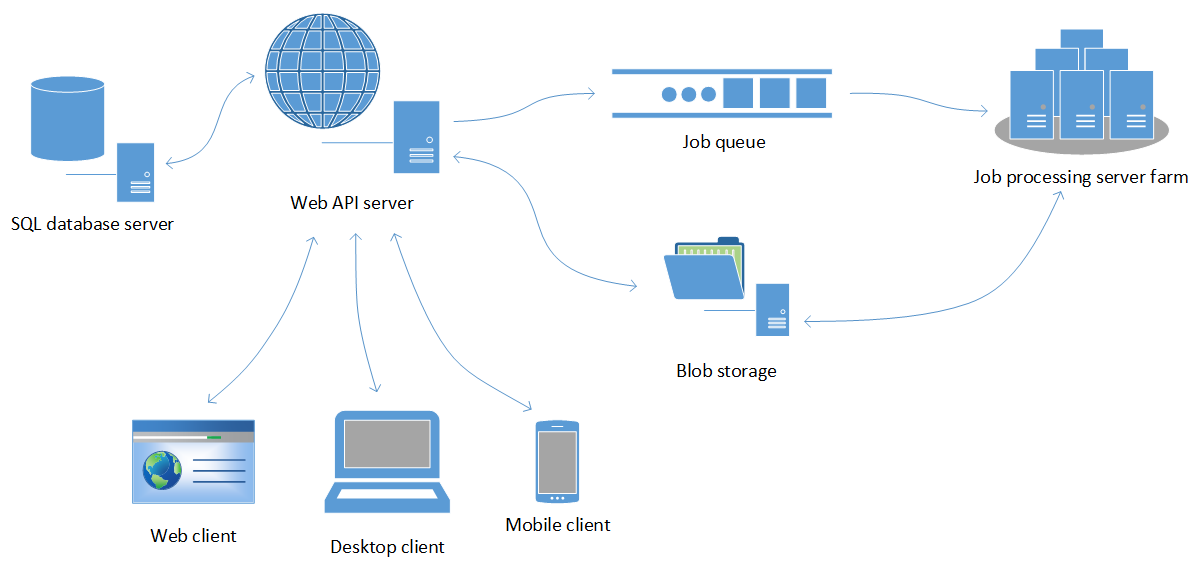
\includegraphics[width=\textwidth]{figures/FEA-architecture}
    \decoRule
    \caption{FEA system architecture.}
    \label{fig:FEA-architecture}
\end{figure}

The architecture relies on an abstraction provided by Platform-as-a-Service\footnote{PaaS. TODO: These services can be carried in a public cloud or on-premises. ...} computing model. No service component is tied directly to a specific machine. Hardware resources are allocated when they are needed by a service infrastructure controller. This makes the scaling and deployment of components easier and allows to focus on the problem domain instead of solving server configuration and networking issues.

To test the prototype implementation of the data management system two client applications are created. The first is the feature-rich desktop post-processor with the support for Microsoft Windows and Linux operating systems. The second is the simple web application that provides basic control over an analysis and basic post-processing capabilities. Its purpose is mainly to demonstrate the benefits of proposed format for results when post-processing complex FEA. Its web-based implementation allows for truly cross-platform experience without the need for installation and allows to access the analysis data even from low-end mobile devices.

The system contains two types of data storage. The relational-database type of storage is intended to store project-related data, user data, and their relationships. 

% toto uloziste rovnez umoznuje reprezentovat vstupni model do analyzy - geometrii a atributy

% meziuloziste urcene pro docasne ulozeni vstupnich a vystupnich souboru z jednotlivych komponent - hlavne mesh generatoru a FEM solveru, protoze cely data management je navrzen nezavisle na pouzitem solveru a generatoru a komponenty, ktere pouzivame v soucasnisti jsou orientovane na vstup a vystup pomoci souboru. V budoucnu predpokladame postupny prechod na prime ukladani vysledku do noveho strukturovaneho formatu a cteni vstupu primo z databaze, kde je ulozeny model - tim odpadne tento mezikrok.

The second type of storage is a blob storage that is used to store file-based data, e.g. input file to FEM solver or output files with results.

% TODO: Two databases. Relational-database to store project-related data and user data. Blob storage to save file-based data (input to mesh generator or FEM solver, output files). Vstup do FEMu (geometricky model v teto architekture muze byt reprezentovan bud vstupnim souborem vygenerovanym v CADu nebo muze byt ulozen)
% In addition to that the desktop postprocessor ma moznost ukladat si data lokalne



% project management, SQL relational database
% zminit modeller a OOFEM-link, ukazka db modelu
% solution.json
% model attributes: viz clanek FEA with Relational DB, section FEA Data and Dataflow

% Pridat diagram prezentujici cely system - vsechny jeho komponenty (Webapi, Solver, Modeller? - misto toho model importer, Web-based postprocessor, Desktop-based postprocessor, Project Database, Result database)

% project-management, storage-format, modeller (OOFEM-link, script-based engine), post-processors, layer format, filters

Figure \ref{fig:FEA-workflow}

\begin{figure}[H]
    \centering
    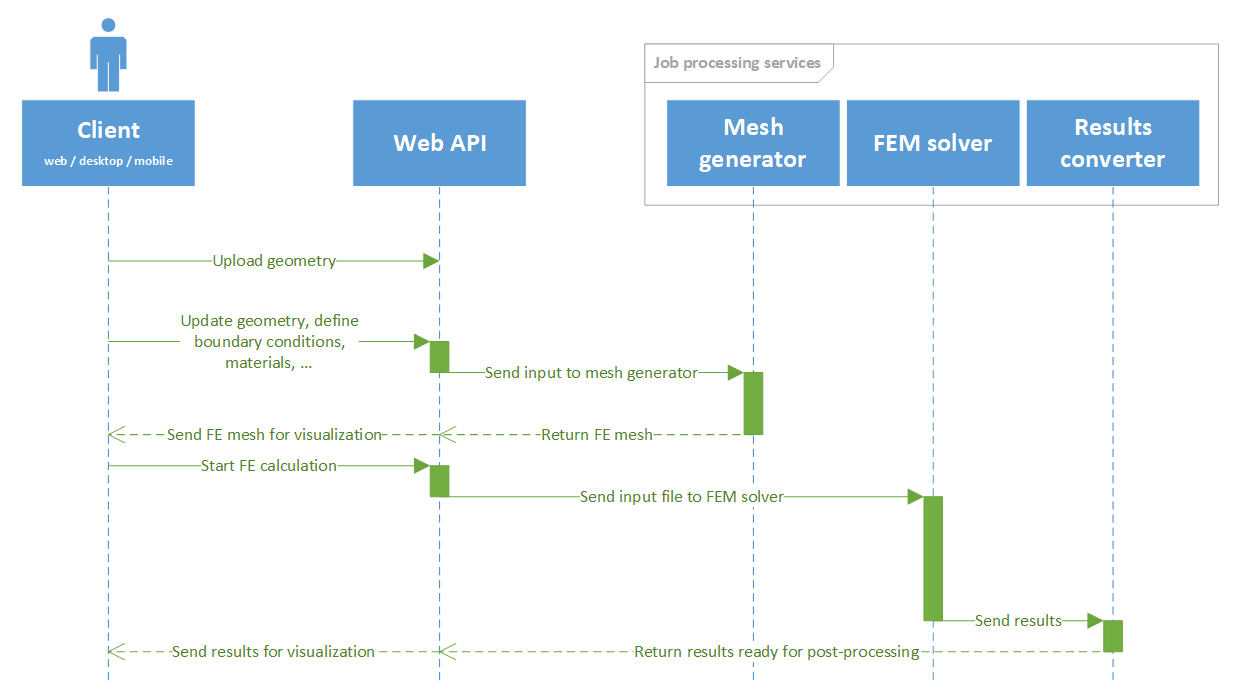
\includegraphics[width=\textwidth]{figures/FEA-workflow}
    \decoRule
    \caption{FEA system workflow.}
    \label{fig:FEA-workflow}
\end{figure}

\section{Project-based data representation}

% Centrem vseho je projekt, projekt ma uzivatele vlastnika a muze mit nekolik dalsich lidi, kteri maji pristup k projektu (ruzna prava, pro cteni ci pro zapis...)
% V ramci jednoho projektu muze byt spusteno vice simulaci, kazda simulace muze mit jiny vstup - at uz geometricky model, atributy, ci jine parametry analyzy. Geometricky model a parametry mohou byt reprezentovany v relacni databazi jak je naznaceno na obrazku \ref{fig:FEA-db-schema}.
% Tento model se da prirozene rozsirit o dalsi entity reprezentujici vysledky simulace, viz Figure Figure \ref{fig:FEA-db-schema-results}. Vysledek simulace reprezentuje entita Solution, ktera obsahuje odkaz na vystupni soubory z FEM solveru. Dale je zde entita Layer reprezentujici transformovane vysledky ze solveru do podoby vhodne pro postprocessing. (Vice v nasledujici kapitole.)

Figure \ref{fig:FEA-db-schema}, Figure \ref{fig:FEA-db-schema-results}

% TODO: add User entity to schema?

\begin{figure}[H]
    \centering
    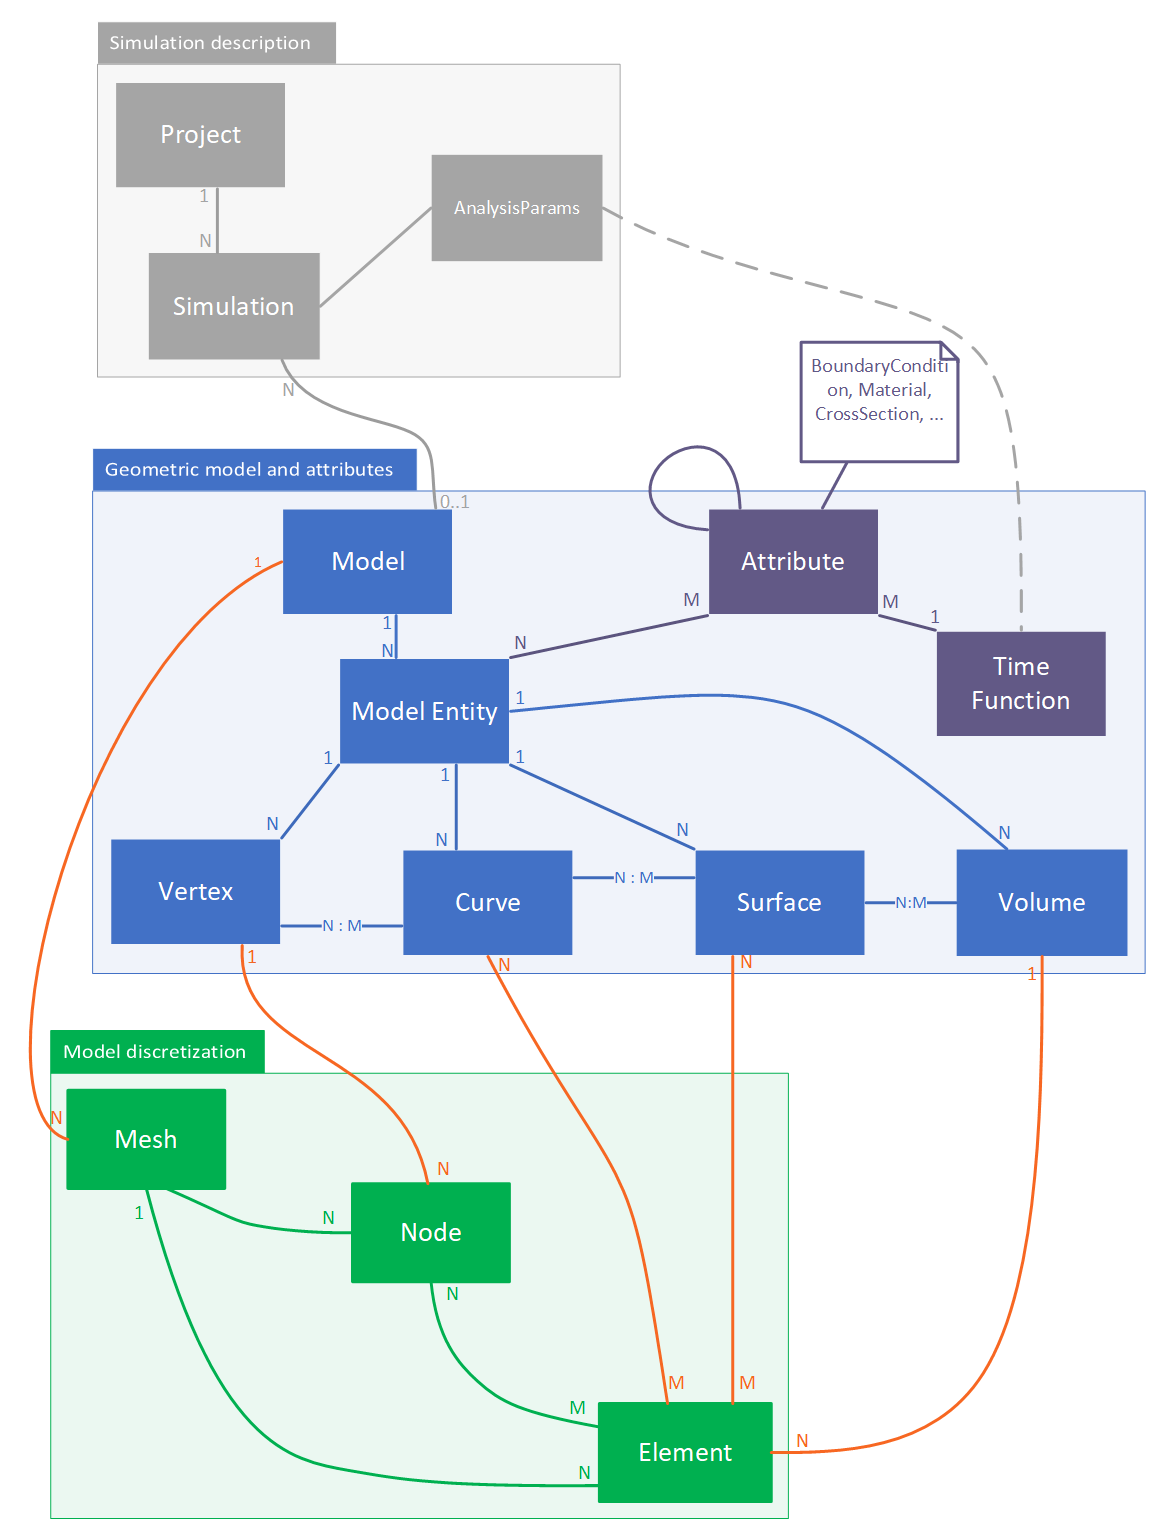
\includegraphics[width=0.8\textwidth]{figures/FEA-database-schema}
    \decoRule
    \caption{Database schema for FEA.}
    \label{fig:FEA-db-schema}
\end{figure}

\begin{figure}[H]
    \centering
    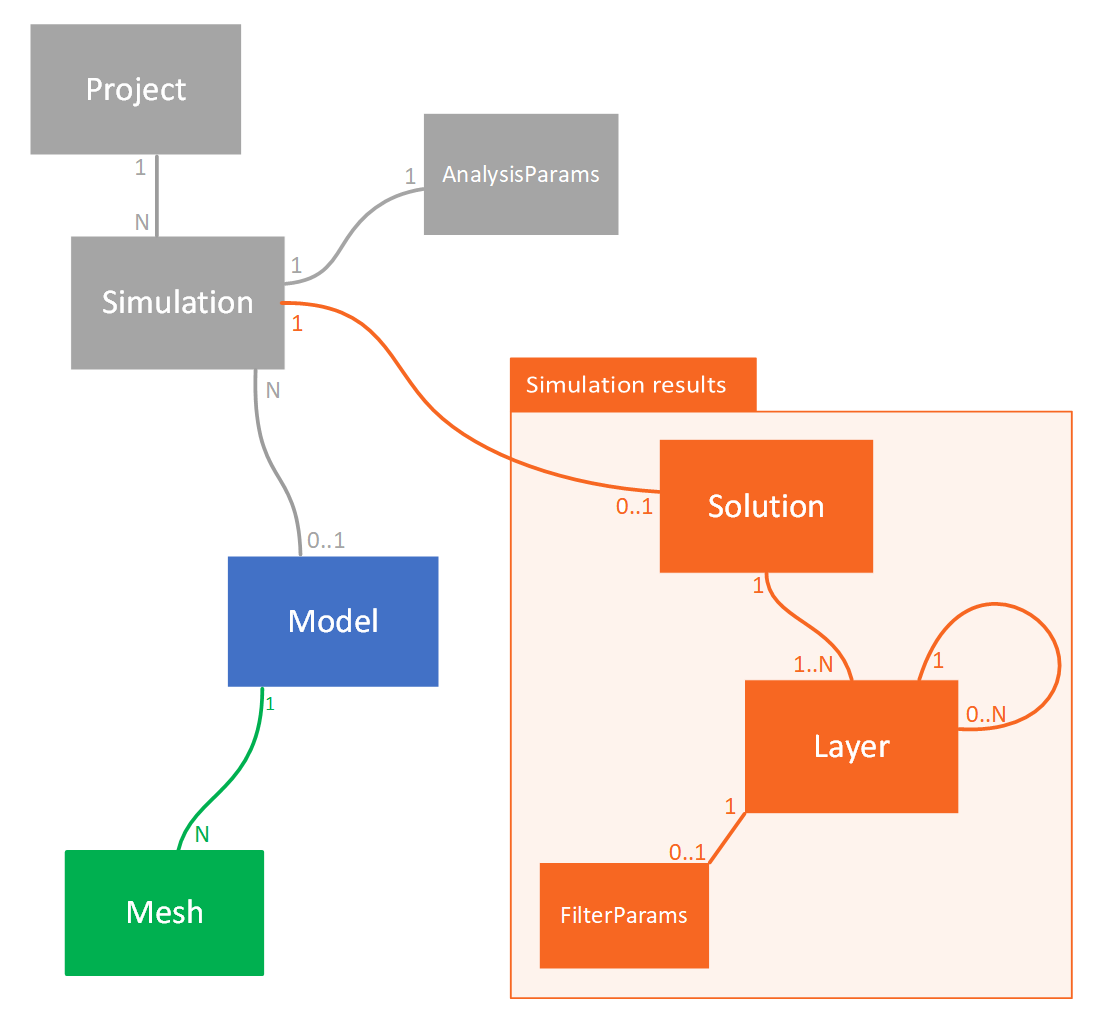
\includegraphics[width=0.7\textwidth]{figures/FEA-database-schema-with-results}
    \decoRule
    \caption{Database schema for FEA with representation of results.}
    \label{fig:FEA-db-schema-results}
\end{figure}

% model and mesh in persistent storage


\section{Storage format for results}
\label{sec:storage-format}

% Result converter component ma za ukol transformovat vysledky z FEM solveru do mojeho formatu (predpokladam pouziti solver komponenty, ktera ma vlastni proprietarni format, protoze se snazim navrhnout system nezavisly na jednotlivych komponentach)

% Centrem vseho je solution. To muze byt reprezentovano entitou v DB. Pripadne solution.json souborem v pripadne vysledku ulozenych a postprocessovanych lokalne. Hlavni koncept pri postprocessingu ke vrstva - layer - reprezentuje sit konecnych prvku a korespondujici vysledky at uz v uzlech ci v prvcich. Tyto data mohou byt zkompresovana. Vysvetlit, proc mam vic vrstev. Proc nestaci jedna.
% TODO: pridat obrazek stromu vrstev.

Figure \ref{fig:layers-tree}

\begin{figure}[H]
    \centering
    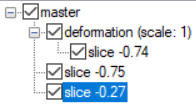
\includegraphics[width=0.5\textwidth]{figures/layers-tree-diagram}
    \decoRule
    \caption{Diagram of layers tree.}
    \label{fig:layers-tree}
\end{figure}

% hodne se inspirovat oznacenymi vetami v clanku FEA-with-relational-DB


% samotny seznam souboru, ktere pouzivam. Nerikat tomu soubory, ale dokumenty? objekty?
% summary.json, mesh.json, attribute.json, and result.json - odkaz do Appendixu na example
% NoSQL DB
% U kazdeho souboru

% konverze z tradicnich souboru do noveho formatu (do budoucna integrovat do solveru); data location Points/Cells/CellPoints, GP extrapolation

% sit je krome vstupu dulezita i u vystupu. je nutne zachovat 1:1 mapovani vysledku na sit

\subsection {Encoding}
% base64, JSON, XML, ...

\subsection {Compression}
% Compression methods: SVD, Wavelet, polynomial functions, ... Kazdou rozepsat, u Wavelet zminit Hilbert curve?
% main features for optimization: key time steps (time step span compression), Randomized SVD, Parallelization, Sparse matrix of details, prenasobeni U matice singularnimi cisly, trochu usetrim pamet, mohu pouzit vzorkovani...

\section{Postprocessing}
\label{sec:postprocessing}

% layers, filters, vytvoreni Surface vrstvy pro webovy postprocessor, barevna skala, Remote/Local solutions - neni rozdil, postprocessor je tenky klient, prepinani skalarnich velicin, vektorove veliciny - je treba nacist vice komponent najednou. Dekomprese: prenasobeni matic - staci jeden radek. ...

\section{Implementation details}
\label{sec:implementation-details}
% implementation details; cloud-infrastructure, Azure functions, web frontend, backend providing project info, blob-storage with layer format; command-based console management - popsat prikazy; reference to appendix with storage format examples
% SVD compression using redsvd; How is realized postprocessing of compressed data
% Encoding: converting to text representation, base64, NaN values, ... UTF8

% Webový browser, WebGL, textové pole se zadáváním příkazů, veškeré zpracování příkazů na serveru, na klient se budou posílat jen grafické buffery

% Přidat podkapitolku o implementaci barevné škály (diskrétní, spojitá, isoareas shader)

Figure \ref{fig:results-class-diagram}.

\begin{figure}[H]
    \centering
    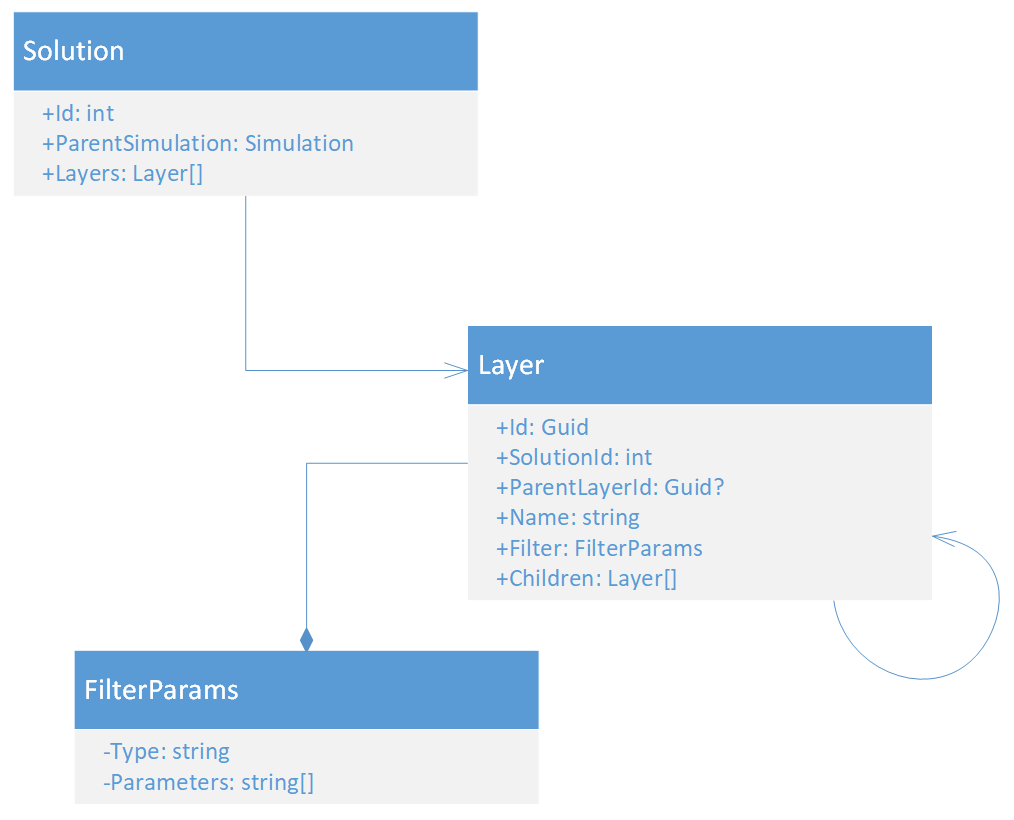
\includegraphics[width=0.7\textwidth]{figures/results-class-diagram}
    \decoRule
    \caption{Class diagram of results representation}
    \label{fig:results-class-diagram}
\end{figure}